\documentclass[semifinal,survey,isne,english]{cpecmu}

%% This is a sample document demonstrating how to use the CPECMU
%% project template. If you are having trouble, see "cpecmu.pdf" for
%% documentation.

\projectNo{P069-1}
\acadyear{2021}

\titleTH{โครงงานสุดเลิฟของฉัน}
\titleEN{Your Project Name Goes Here}

\author{นายปิยวุฒิ บุญเจริญ}{Kinnaree Tirelumlert}{690610696}
\author{นายบรรจบ พบเอฟตลอด}{Banjob Pob-eftalord}{690610969}

\cpeadvisor{chinawat}
\cpecommittee{paskorn}
\committee{รศ.ดร.\,นิพนธ์ ธีรอำพน}{Assoc.\,Prof.\,Nipon Theera-Umpon, Ph.D.}

%% Some possible packages to include:
\usepackage[final]{graphicx} % for including graphics

%% Add bookmarks and hyperlinks in the document.
\PassOptionsToPackage{hyphens}{url}
\usepackage[colorlinks=true,allcolors=Blue4,citecolor=red,linktoc=all]{hyperref}
\def\UrlLeft#1\UrlRight{$#1$}

%% Needed just by this example, but maybe not by most reports
\usepackage{afterpage} % for outputting
\usepackage{pdflscape} % for landscape figures and tables. 

%% Some other useful packages. Look these up to find out how to use
%% them.
% \usepackage{natbib}    % for author-year citation styles
% \usepackage{txfonts}
% \usepackage{appendix}  % for appendices on a per-chapter basis
% \usepackage{xtab}      % for tables that go over multiple pages
% \usepackage{subfigure} % for subfigures within a figure
% \usepackage{pstricks,pdftricks} % for access to special PostScript and PDF commands
% \usepackage{nomencl}   % if you have a list of abbreviations

%% if you're having problems with overfull boxes, you may need to increase
%% the tolerance to 9999
% \tolerance=9999

\bibliographystyle{plain}
% \bibliographystyle{IEEEbib}

% \renewcommand{\topfraction}{0.85}
% \renewcommand{\textfraction}{0.1}
% \renewcommand{\floatpagefraction}{0.75}

%% Example for glossary entry
%% Need to use glossary option
%% See glossaries package for complete documentation.
\ifglossary
  \newglossaryentry{lorem ipsum}{
    name=lorem ipsum,
    description={derived from Latin dolorem ipsum, translated as ``pain itself''}
  }
\fi

%% Uncomment this command to preview only specified LaTeX file(s)
%% imported with \include command below.
%% Any other file imported via \include but not specified here will not
%% be previewed.
%% Useful if your report is large, as you might not want to build
%% the entire file when editing a certain part of your report.
% \includeonly{chapters/intro,chapters/background}

\begin{document}
\maketitle
\makesignature

\ifproject
\begin{abstractTH}
LoRa (Long Range) is a low-power wireless communication technology widely used in Internet of Things (IoT) applications. These include environmental monitoring, agriculture, and infrastructure systems. While LoRa excels in long-range communication, it lacks native security features. Data transmitted over LoRa can be intercepted, and hardcoded encryption keys on microcontrollers like the ESP32 are vulnerable to extraction via physical access. This poses a serious security threat to the IoT network. 
 
This project presents a secure communication framework for IoT systems using LoRa and MicroPython, focusing on lightweight encryption and key management. Data transmissions are encrypted using the cryptolib module, and session keys are updated based on shared physical metrics such as RSSI values and communication response timing. These metrics are known only to the legitimate communicating devices which  increases resistance to message interception and spoofing. The approach is designed for resource-constrained and physically exposed environments. It provides a practical solution for securing IoT communications without compromising performance or power efficiency.
\end{abstractTH}

\begin{abstract}
LoRa (Long Range) is a low-power wireless communication technology widely used in Internet of Things (IoT) applications. These include environmental monitoring, agriculture, and infrastructure systems. While LoRa excels in long-range communication, it lacks native security features. Data transmitted over LoRa can be intercepted, and hardcoded encryption keys on microcontrollers like the ESP32 are vulnerable to extraction via physical access. This poses a serious security threat to the IoT network. 
 
This project presents a secure communication framework for IoT systems using LoRa and MicroPython, focusing on lightweight encryption and key management. Data transmissions are encrypted using the cryptolib module, and session keys are updated based on shared physical metrics such as RSSI values and communication response timing. These metrics are known only to the legitimate communicating devices which  increases resistance to message interception and spoofing. The approach is designed for resource-constrained and physically exposed environments. It provides a practical solution for securing IoT communications without compromising performance or power efficiency.

\end{abstract}

\iffalse
\begin{dedication}
This document is dedicated to all Chiang Mai University students.

Dedication page is optional.
\end{dedication}
\fi % \iffalse

\begin{acknowledgments}
Your acknowledgments go here. Make sure it sits inside the
\texttt{acknowledgment} environment.

\acksign{2020}{5}{25}
\end{acknowledgments}%
\fi % \ifproject

\contentspage

\ifproject
\figurelistpage

\tablelistpage
\fi % \ifproject

% \abbrlist % this page is optional

% \symlist % this page is optional

% \preface % this section is optional


\pagestyle{empty}\cleardoublepage
\normalspacing \setcounter{page}{1} \pagenumbering{arabic} \pagestyle{cpecmu}

\chapter{\ifenglish Introduction\else บทนำ\fi}

\section{\ifenglish Project rationale\else ที่มาของโครงงาน\fi}

\section{\ifenglish Objectives\else วัตถุประสงค์ของโครงงาน\fi}
\begin{enumerate}
    \item
\end{enumerate}

\section{\ifenglish Project scope\else ขอบเขตของโครงงาน\fi}

\subsection{\ifenglish Hardware scope\else ขอบเขตด้านฮาร์ดแวร์\fi}

\subsection{\ifenglish Software scope\else ขอบเขตด้านซอฟต์แวร์\fi}

\section{\ifenglish Expected outcomes\else ประโยชน์ที่ได้รับ\fi}

\section{\ifenglish Technology and tools\else เทคโนโลยีและเครื่องมือที่ใช้\fi}

\subsection{\ifenglish Hardware technology\else เทคโนโลยีด้านฮาร์ดแวร์\fi}

\subsection{\ifenglish Software technology\else เทคโนโลยีด้านซอฟต์แวร์\fi}

\section{\ifenglish Project plan\else แผนการดำเนินงาน\fi}

% \begin{plan}{6}{2020}{2}{2021}
%     \planitem{7}{2020}{8}{2020}{ศึกษาค้นคว้า}
%     \planitem{8}{2020}{1}{2021}{ชิล}
%     \planitem{2}{2021}{2}{2021}{เผา}
%     \planitem{12}{2019}{1}{2022}{ทดสอบ}
% \end{plan}

\section{\ifenglish Roles and responsibilities\else บทบาทและความรับผิดชอบ\fi}
% อธิบายว่าในการทำงาน นศ. มีการกำหนดบทบาทและแบ่งหน้าที่งานอย่างไรในการทำงาน จำเป็นต้องใช้ความรู้ใดในการทำงานบ้าง

\section{\ifenglish%
Impacts of this project on society, health, safety, legal, and cultural issues
\else%
ผลกระทบด้านสังคม สุขภาพ ความปลอดภัย กฎหมาย และวัฒนธรรม
\fi}

% แนวทางและโยชน์ในการประยุกต์ใช้งานโครงงานกับงานในด้านอื่นๆ รวมถึงผลกระทบในด้านสังคมและสิ่งแวดล้อมจากการใช้ความรู้ทางวิศวกรรมที่ได้

\chapter{\ifenglish Background Knowledge and Theory\else ทฤษฎีที่เกี่ยวข้อง\fi}

% การทำโครงงาน เริ่มต้นด้วยการศึกษาค้นคว้า ทฤษฎีที่เกี่ยวข้อง หรือ งานวิจัย/โครงงาน ที่เคยมีผู้นำเสนอไว้แล้ว ซึ่งเนื้อหาในบทนี้ก็จะเกี่ยวกับการอธิบายถึงสิ่งที่เกี่ยวข้องกับโครงงาน เพื่อให้ผู้อ่านเข้าใจเนื้อหาในบทถัดๆ ไปได้ง่ายขึ้น

\section{Internet of Things (IoT)}
The Internet of Things (IoT) refers to a network of interconnected devices that can sense, process, and exchange data with minimal human intervention. These devices are widely deployed in applications such as smart homes, healthcare monitoring, environmental sensing, transportation systems, and industrial automation. While IoT enables efficiency and automation, it also introduces security challenges. Many IoT devices are resource-constrained in terms of processing power, memory, and energy supply, making it difficult to implement traditional, computation-heavy cryptographic techniques. As a result, IoT networks are often vulnerable to attacks such as eavesdropping, replay, and message injection.

\section{LoRa Technology}
LoRa (Long Range) is a low-power wide-area network (LPWAN) communication technology that enables devices to transmit data over several kilometers while consuming minimal energy. This makes it suitable for IoT applications where devices must operate on battery power for extended periods. LoRa achieves long-distance communication using Chirp Spread Spectrum (CSS) modulation, which provides robustness against noise and interference.
 However, LoRa’s primary limitation is its lack of built-in security mechanisms. The physical layer itself does not provide strong confidentiality or integrity protection. While LoRaWAN (the higher-layer protocol) introduces some security features, lightweight LoRa implementations—such as those used in simple ESP32 + LoRa projects—are highly vulnerable to interception, spoofing, and key extraction if insecure practices (e.g., hardcoded keys) are used.

 \section{Received Signal Strength Indicator (RSSI)}
 The Received Signal Strength Indicator (RSSI) measures the power level of a received wireless signal, typically expressed in decibels relative to one milliwatt (dBm). In LoRa systems, RSSI is automatically measured at the receiver whenever a packet is received. Normally, RSSI is used to evaluate link quality or assist in adaptive communication strategies.
 In the context of security, RSSI can also be leveraged as a source of entropy for key generation. Since RSSI values fluctuate depending on distance, obstacles, interference, and environmental conditions, they are inherently dynamic and difficult for an attacker to predict without being physically co-located in the communication channel. By using RSSI values as a basis for session key generation, IoT devices can avoid reliance on static, pre-shared keys that are easy to compromise.
\section{ Lightweight Cryptography}
Lightweight cryptography refers to cryptographic techniques designed specifically for devices with limited computational and memory resources. Unlike traditional algorithms such as AES-256 or RSA, which require significant processing power, lightweight algorithms are optimized for efficiency while maintaining an acceptable level of security. Typical strategies include reducing key sizes, minimizing memory overhead, or designing algorithms tailored for 8-bit or 32-bit microcontrollers.
 For IoT applications using devices like the ESP32, lightweight cryptography is essential to balance security with system performance. The challenge is to implement schemes that protect data confidentiality and integrity without exceeding constraints such as 10 KB of program memory or 300 bytes of RAM.
\section{Key Management in IoT}
Key management is one of the most critical aspects of securing IoT networks. Traditional approaches rely on pre-shared static keys, which pose significant risks: once an attacker obtains the key, they can decrypt all subsequent communications. Dynamic key management schemes provide stronger protection by regularly updating session keys.
 One promising approach is to derive session keys from physical-layer metrics, such as RSSI. Since each device independently measures RSSI during communication, keys can be generated locally without transmitting sensitive information over the air. To ensure synchronization, both devices agree on an adjustment interval and use a shared keyword for verification. This method significantly reduces the risk of interception and makes it difficult for attackers to reuse keys, thereby enhancing overall IoT security.

\subsection{Subsection heading goes here}

Subsection 1 text

\subsubsection{Subsubsection 1 heading goes here}
Subsubsection 1 text

\subsubsection{Subsubsection 2 heading goes here}
Subsubsection 2 text

\section{Third section}
Section 3 text. The dielectric constant\index{dielectric constant}
at the air-metal interface determines
the resonance shift\index{resonance shift} as absorption or capture occurs
is shown in Equation~\eqref{eq:dielectric}:

\begin{equation}\label{eq:dielectric}
k_1=\frac{\omega}{c({1/\varepsilon_m + 1/\varepsilon_i})^{1/2}}=k_2=\frac{\omega
\sin(\theta)\varepsilon_\mathit{air}^{1/2}}{c}
\end{equation}

\noindent
where $\omega$ is the frequency of the plasmon, $c$ is the speed of
light, $\varepsilon_m$ is the dielectric constant of the metal,
$\varepsilon_i$ is the dielectric constant of neighboring insulator,
and $\varepsilon_\mathit{air}$ is the dielectric constant of air.

\section{About using figures in your report}

% define a command that produces some filler text, the lorem ipsum.
\newcommand{\loremipsum}{
  \textit{Lorem ipsum dolor sit amet, consectetur adipisicing elit, sed do
  eiusmod tempor incididunt ut labore et dolore magna aliqua. Ut enim ad
  minim veniam, quis nostrud exercitation ullamco laboris nisi ut
  aliquip ex ea commodo consequat. Duis aute irure dolor in
  reprehenderit in voluptate velit esse cillum dolore eu fugiat nulla
  pariatur. Excepteur sint occaecat cupidatat non proident, sunt in
  culpa qui officia deserunt mollit anim id est laborum.}\par}

\begin{figure}
  \centering

  \fbox{
     \parbox{.6\textwidth}{\loremipsum}
  }

  % To include an image in the figure, say myimage.pdf, you could use
  % the following code. Look up the documentation for the package
  % graphicx for more information.
  % \includegraphics[width=\textwidth]{myimage}

  \caption[Sample figure]{This figure is a sample containing \gls{lorem ipsum},
  showing you how you can include figures and glossary in your report.
  You can specify a shorter caption that will appear in the List of Figures.}
  \label{fig:sample-figure}
\end{figure}

Using \verb.\label. and \verb.\ref. commands allows us to refer to
figures easily. If we can refer to Figures
\ref{fig:walrus} and \ref{fig:sample-figure} by name in the {\LaTeX}
source code, then we will not need to update the code that refers to it
even if the placement or ordering of the figures changes.

\loremipsum\loremipsum

% This code demonstrates how to get a landscape table or figure. It
% uses the package lscape to turn everything but the page number into
% landscape orientation. Everything should be included within an
% \afterpage{ .... } to avoid causing a page break too early.
\afterpage{
  \begin{landscape}
  \begin{table}
    \caption{Sample landscape table}
    \label{tab:sample-table}

    \centering

    \begin{tabular}{c||c|c}
        Year & A & B \\
        \hline\hline
        1989 & 12 & 23 \\
        1990 & 4 & 9 \\
        1991 & 3 & 6 \\
    \end{tabular}
  \end{table}
  \end{landscape}
}

\loremipsum\loremipsum\loremipsum

\section{Overfull hbox}

When the \verb.semifinal. option is passed to the \verb.cpecmu. document class,
any line that is longer than the line width, i.e., an overfull hbox, will be
highlighted with a black solid rule:
\begin{center}
\begin{minipage}{2em}
juxtaposition
\end{minipage}
\end{center}

\section{\ifenglish%
\ifcpe CPE \else ISNE \fi knowledge used, applied, or integrated in this project
\else%
ความรู้ตามหลักสูตรซึ่งถูกนำมาใช้หรือบูรณาการในโครงงาน
\fi
}

% อธิบายถึงความรู้ และแนวทางการนำความรู้ต่างๆ ที่ได้เรียนตามหลักสูตร ซึ่งถูกนำมาใช้ในโครงงาน

\section{\ifenglish%
Extracurricular knowledge used, applied, or integrated in this project
\else%
ความรู้นอกหลักสูตรซึ่งถูกนำมาใช้หรือบูรณาการในโครงงาน
\fi
}

% อธิบายถึงความรู้ต่างๆ ที่เรียนรู้ด้วยตนเอง และแนวทางการนำความรู้เหล่านั้นมาใช้ในโครงงาน

\chapter{\ifproject%
\ifenglish Project Structure and Methodology\else โครงสร้างและขั้นตอนการทำงาน\fi
\else%
\ifenglish Project Structure\else โครงสร้างของโครงงาน\fi
\fi
}

% ในบทนี้จะกล่าวถึงหลักการ และการออกแบบระบบ

\makeatletter

% \renewcommand\section{\@startsection {section}{1}{\z@}%
%                                    {13.5ex \@plus -1ex \@minus -.2ex}%
%                                    {2.3ex \@plus.2ex}%
%                                    {\normalfont\large\bfseries}}

\makeatother
%\vspace{2ex}
% \titleformat{\section}{\normalfont\bfseries}{\thesection}{1em}{}
% \titlespacing*{\section}{0pt}{10ex}{0pt}

\section{Methodology}

\subsection{System Architecture}
 The proposed framework consists of two ESP32 devices, each connected to a LoRa SX1276 module. One device operates as the sender (initiator), and the other as the receiver (responder). The devices communicate over LoRa to exchange verification and application messages. The overall architecture ensures that both devices can generate identical session keys without directly transmitting key material.

\begin{figure}[htbp]
\begin{center}
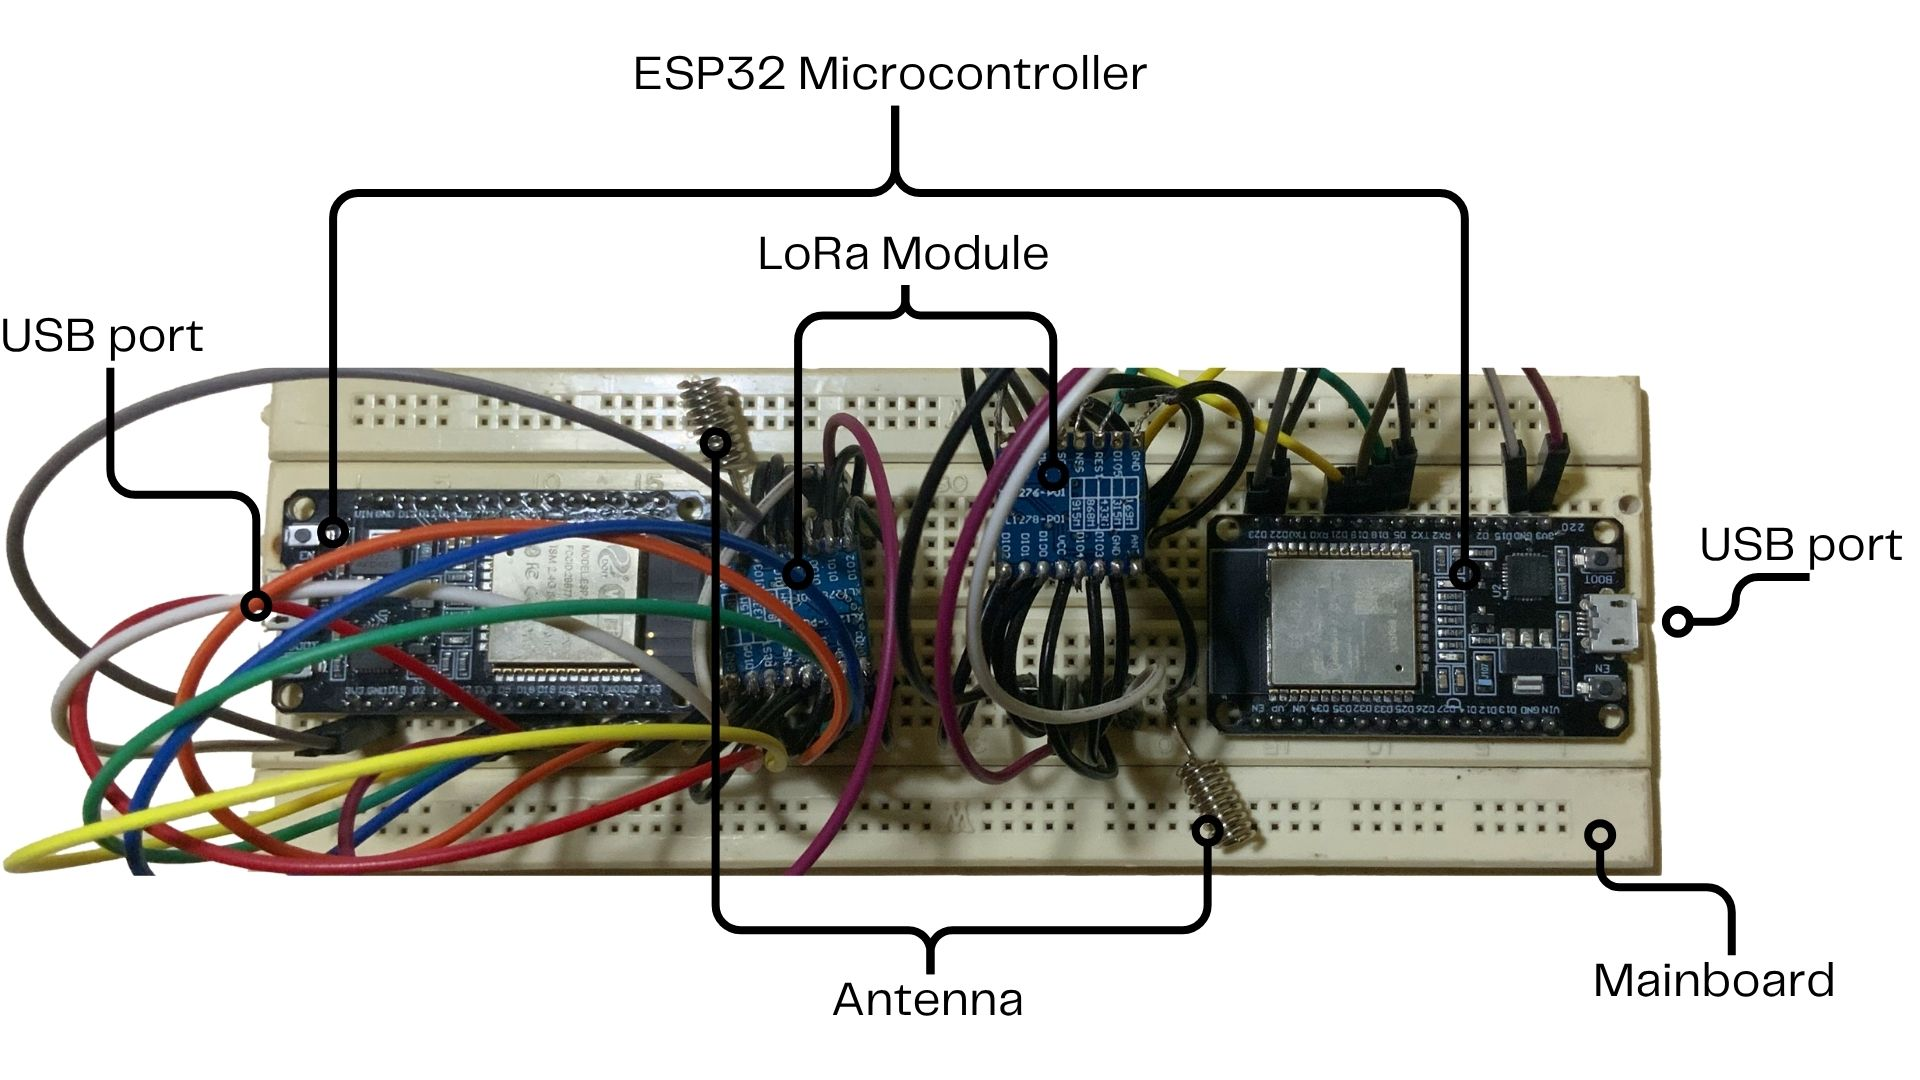
\includegraphics[width=0.8\textwidth]{Architecture.jpg}
\end{center}
\caption[Picture]{Design Architecture}
\label{fig:architecture}
\end{figure}

\subsection{RSSI-Based Key Generation}
To synchronize RSSI values, one device (the initiator) first transmits a known verification message. The receiving device measures the RSSI of this signal and attempts to decode the message using its reading. If decryption fails, the receiver iteratively adjusts its interpretation by shifting the RSSI value up or down within a pre-agreed tolerance interval (e.g., ±0.5 dBm) until the message is correctly decrypted. Unlike static pre-shared keys, which remain fixed and are vulnerable once compromised, session keys in this framework are dynamically derived from RSSI. Since RSSI is measured uniquely at the receiver and varies naturally with the environment, it is difficult for an attacker to predict or replicate. Security is further enhanced by concatenating the RSSI values and sampling them across multiple frequency channels into an array. 

\subsection{Keyword Verification}
To ensure correctness, both devices share a pre-defined keyword. After decryption, the receiver compares the result against this keyword. A match confirms that both devices are synchronized on the same session key. If the keyword is not matched, the process repeats until a valid session key is established.

\subsection{System Implementation}

\subsubsection{Hardware Setup}
The following components are required for the system implementation:
\begin{itemize}
    \item ESP32 development board (MicroPython-compatible)
    \item SX1276 LoRa module
    \item USB cable for ESP32
    \item Jumper wires
    \item Computer with \texttt{esptool.py} and \texttt{mpremote} installed
\end{itemize}

\subsubsection{Pin Mapping}
The interfacing between the ESP32 and the SX1276 module is established through the SPI bus and control lines.  
The pin assignments are listed in Table~\ref{tab:pinmapping}. These may be modified in \texttt{lora.py} as required.

\begin{table}[htbp]
\centering
\label{tab:pinmapping}
\begin{tabular}{|c|c|}
\hline
\textbf{Signal} & \textbf{ESP32 GPIO Pin} \\ \hline
MISO & GPIO19 \\ \hline
MOSI & GPIO23 \\ \hline
SCK  & GPIO18 \\ \hline
CS   & GPIO5  \\ \hline
RST  & GPIO17 \\ \hline
DIO0 & GPIO26 \\ \hline
\end{tabular}
\caption{Pin Mapping between ESP32 and LoRa Module}
\end{table}

\subsection{Flashing MicroPython on ESP32}

To run the ESP32 with MicroPython, follow these steps:

\subsubsection{Erase Existing Flash}
Before flashing, erase the current firmware on the ESP32:

\begin{verbatim}
esptool --port COM6 erase_flash
\end{verbatim}

\noindent This clears the flash memory of a standard ESP32.

\subsubsection{Write MicroPython Firmware}
Next, write the MicroPython firmware to the ESP32. Replace {<micropython-firmware.bin>} with your firmware file name:

\begin{verbatim}
esptool --baud 460800 write_flash 0 \
ESP32_GENERIC_C6-20250415-v1.25.0.bin
\end{verbatim}


\noindent Example using a specific firmware file:

\begin{verbatim}
esptool --baud 460800 write_flash 0 ESP32_GENERIC_C6-20250415-v1.25.0.bin
\end{verbatim}

\noindent After flashing, the ESP32 is ready to run MicroPython scripts via a serial connection.

\subsection{Prepare and Upload Files}

Before running the system, edit the \texttt{lora.py} file locally to ensure the pin mapping matches your ESP32 configuration (see Section~\ref{tab:pinmapping}).

\subsubsection{Upload \texttt{lora.py} to ESP32}
Use \texttt{mpremote} to upload the Python script to the ESP32:

\begin{verbatim}
mpremote connect COM6 fs cp lora.py 
\end{verbatim}

\noindent Explanation:
\begin{itemize}
    \item \texttt{mpremote connect COM6} — Connects to the ESP32 on port COM6.
    \item \texttt{fs cp lora.py :} — Copies the \texttt{lora.py} file to the root directory of the ESP32 filesystem.
\end{itemize}

After uploading, the ESP32 is ready to run the LoRa communication program.

\subsection{Connect to Shell and Run}

After uploading the necessary files, follow these steps to execute the program on the ESP32 nodes.

\begin{enumerate}
    \item Connect the ESP32 to your computer via USB.
    
    \item Open the serial REPL using \texttt{mpremote}:

\begin{verbatim}
mpremote connect /dev/ttyUSB0 repl
\end{verbatim}
    
    \item Upload and run the application scripts:
    \begin{itemize}
        \item On Node A (sender): upload and run \texttt{sender.py}.
        \item On Node B (receiver): upload and run \texttt{receiver.py}.
    \end{itemize}
\end{enumerate}

Once both nodes are running, they can communicate over LoRa, exchange verification messages, and generate session keys dynamically.

\subsection{LoRa Communication Script}

The following Python script (\texttt{sender.py}) demonstrates sending and receiving LoRa packets using the SX1276 module on an ESP32. It includes unicast requests, broadcast messages, and handling of packet reception.

\subsection{LoRa Communication Script}

The following Python script (\texttt{sender.py}) demonstrates sending and receiving LoRa packets using the SX1276 module on an ESP32. It includes unicast requests, broadcast messages, and handling of packet reception.
{\scriptsize
\begin{verbatim}
from machine import Pin
import time, urandom as random
from lora import SX1276

# Pin configuration
LoRa_MISO_Pin = 19
LoRa_MOSI_Pin = 23
LoRa_SCK_Pin  = 18
LoRa_CS_Pin   = 5
LoRa_RST_Pin  = 17
LoRa_DIO0_Pin = 27
LoRa_DIO1_Pin = 35
LoRa_DIO2_Pin = 34
SPI_CH        = 2  # VSPI

# Random channel hopping setup
random.seed(11)
channels2Hopping = [914_000_000 + 200_000 * random.randint(0, 10) for i in range(128)]  # 914~916 MHz

LoRa_id = 1
lora = SX1276(LoRa_RST_Pin, LoRa_CS_Pin, SPI_CH, LoRa_SCK_Pin, LoRa_MOSI_Pin, LoRa_MISO_Pin,
              LoRa_DIO0_Pin, LoRa_DIO1_Pin, LoRa_id, channels2Hopping, debug=False)

# Packet reception handler
def get_payload(self, data, SNR, RSSI):
    global received_payload
    received_payload = data

lora.req_packet_handler = get_payload

###########################################
# First REQ packet
###########################################
payload = str(random.randint(100,65536)) + ") Hello~"
print('[Sending]', payload)
lora.send(dst_id=0, msg=payload, pkt_type=lora.PKT_TYPE['REQ'])
while not lora.is_available:
    time.sleep(1)

###########################################
# Two-way communication (receive)
###########################################
received_payload = None
lora.mode = 'RXCONTINUOUS'
while not lora.is_available:
    time.sleep(1)
print('[Received] What we receive from the receiver is:', received_payload)

###########################################
# Send REQ packet to wrong receiver
###########################################
payload = str(random.randint(100,65536)) + ") You will not receive this packet because we specified a wrong dst_id"
print('[Sending]', payload)
lora.send(dst_id=3, msg=payload, pkt_type=lora.PKT_TYPE['REQ'], timeout=10, retry=3, debug=True)

for i in range(10):
    if lora.is_available: break
    time.sleep(1)
else:
    print("[Note] you will see this line because lora.is_available is always false")

###########################################
# Send broadcast packets
###########################################
time.sleep(10)
payload = str(random.randint(100,65536)) + ") This long BRD packet will be received"
print('[Sending]', payload)
lora.send(dst_id=0, msg=payload, pkt_type=lora.PKT_TYPE['BRD'])

time.sleep(10)
payload = str(random.randint(100,65536)) + ") This long BRD packet will also be received 
print('[Sending]', payload)
lora.send(dst_id=3, msg=payload, pkt_type=lora.PKT_TYPE['BRD'])
\end{verbatim}
}
This script demonstrates:
\begin{itemize}
    \item Sending a unicast request packet (\texttt{REQ}) to a specific node.
    \item Receiving packets and handling RSSI/SNR values.
    \item Handling cases where the destination ID is incorrect.
    \item Sending broadcast (\texttt{BRD}) packets that are received by all nodes, regardless of the destination ID.
\end{itemize}

\subsection{Receiver Node Script}

The following Python script (\texttt{receiver.py}) demonstrates the ESP32 receiving LoRa packets, replying to unicast requests, and handling broadcast packets.
{\scriptsize
\begin{verbatim}
from machine import Pin
import time, urandom as random
from lora import SX1276

# Pin configuration
LoRa_MISO_Pin = 19
LoRa_MOSI_Pin = 23
LoRa_SCK_Pin  = 18
LoRa_CS_Pin   = 5
LoRa_RST_Pin  = 17
LoRa_DIO0_Pin = 27
LoRa_DIO1_Pin = 35
LoRa_DIO2_Pin = 34
SPI_CH        = 2  # VSPI

# Channel hopping setup (both sender and receiver must know the sequence)
random.seed(11)
channels2Hopping = [914_000_000 + 200_000 * random.randint(0,10) for i in range(128)]

LoRa_id = 0
lora = SX1276(LoRa_RST_Pin, LoRa_CS_Pin, SPI_CH, LoRa_SCK_Pin, LoRa_MOSI_Pin, LoRa_MISO_Pin,
LoRa_DIO0_Pin, LoRa_DIO1_Pin, LoRa_id, channels2Hopping, debug=False)

# Packet handlers
def get_payload(self, data, SNR, RSSI):
    global received_payload
    received_payload = data

lora.req_packet_handler = get_payload
lora.brd_packet_handler = lambda self, data, SNR, RSSI: print("[BRD]", data)

###########################################
# Prepare to receive first REQ packet
###########################################
received_payload = None
lora.mode = 'RXCONTINUOUS'
while not lora.is_available:
    time.sleep(1)

print("[Note] We will see this line after receiver ACKed the first REQ packet with an ACK packet. "
      "Then the receiver becomes the new sender.")

# Reply to 'Hello~' packet
print('[Received]', received_payload)
if received_payload[-6:] != b'Hello~': raise

payload = str(random.randint(100,65536)) + ") Hi ~ I have received your hello"
lora.send(dst_id=1, msg=payload, pkt_type=lora.PKT_TYPE['REQ'])
print('[Sending]', payload)
while not lora.is_available:  # Stop if our reply got acknowledged
    time.sleep(1)

###########################################
# Prepare to receive two BRD packets
###########################################
received_payload = None
lora.mode = 'RXCONTINUOUS'
while not lora.is_available:
    time.sleep(1)

print("[Note] This line will not be reached because BRD is not two-way communication. "
      "The receiver will not stop listening.")
\end{verbatim}
}

\begin{itemize}
    \item Continuous reception of REQ packets.
    \item Replying to a unicast request (two-way communication).
    \item Handling broadcast (BRD) packets, which are received but do not trigger acknowledgment.
\end{itemize}


\chapter{\ifproject%
\ifenglish Experimentation and Results\else การทดลองและผลลัพธ์\fi
\else%
\ifenglish System Evaluation\else การประเมินระบบ\fi
\fi}

\section{Evaluation Metrics}
If implemented, the proposed framework would be evaluated using the following criteria:

\subsection{Performance}
 the time required for key generation, encryption, and decryption on ESP32 devices.

\subsection{Resource Usage}
 memory and CPU consumption, ensuring the design remains lightweight.

\subsection{Security Assessment}
 resistance against common IoT attacks, including replay and man-in-the-middle (MITM) attacks.

 \section{Evaluation Method}

\subsection{Correctness Testing}
Repeatedly transmit verification messages and record the percentage of times the receiver derives the correct key and matches the predefined keyword.

\subsection{Performance Measurement}
Measure execution time of key generation and encryption/decryption functions using built-in timers on ESP32.

\subsection{Resource Usage}
Monitor program memory footprint and RAM usage to ensure they remain under the target limits (~10 KB flash, ~300 bytes RAM).

\subsection{Security Testing}
Simulate potential attack scenarios such as replaying old packets or attempting to intercept communication, to evaluate whether the dynamic key mechanism prevents message reuse or prediction.

 \section{Evaluation Method}
 The evaluation is expected to show that the RSSI-based key generation approach achieves high correctness in key agreement, maintains lightweight resource usage suitable for ESP32 devices, and provides improved resilience against interception compared to static key methods.

\section{Comparative Discussion with Related Works}

To assess the contribution of the proposed RSSI-based lightweight secure communication framework, it is useful to compare it with recent research in LoRa security.

\subsubsection{Chaos and Timing Approaches}
Erkan et al. (2023) proposed a chaos-based encryption with a timing confirmation algorithm on LoRa. They use a Logistic map as a pseudo-random generator and millisecond-level timing signals for message validation. Their evaluation, including NIST randomness and entropy tests, shows that chaotic keys provide high unpredictability. This study, however, focuses on theoretical analysis of randomness and timing rather than memory or CPU usage constraints~\cite{erkan2023secure}.

\subsubsection{Lightweight Block Cipher on ESP32}
Lim et al. (2024) designed a lightweight block cipher for ESP32 based on AES/DES principles. The algorithm uses custom S-boxes and P-boxes for encryption and is validated through SAC, monobit, and correlation tests. It demonstrates feasibility on ESP32 with approximately 3 ms execution time per encryption and randomness performance close to optimal. However, it depends on static pre-shared keys, increasing complexity in key management~\cite{ni2024esp32crypto}.

\subsubsection{Frequency-Hopping Network Architectures}
    Ortigoso et al. (2024) introduced Dynamic Dual Frequency Hopping (DDFH), a network-level architecture using dual radios and mesh topology to improve scalability and mitigate eavesdropping. Their solution achieved a $\sim 94.66\%$ packet success rate in prototypes. While effective, DDFH targets large-scale LoRaWAN deployments with Raspberry Pi and dual-antenna hardware. In contrast, our approach is device-centric, requiring only low-cost ESP32 and LoRa modules~\cite{ortigoso2024ddfh}.

\subsubsection{Physical-Layer RSSI + CRT Encryption}
Zhang et al. (2021) proposed a physical-layer scheme combining RSSI-based key extraction with the Chinese Remainder Theorem (CRT) to generate cyclic shift encryption factors. Their algorithm preserves BER performance while degrading eavesdropper decoding to near 0.5 BER. Our work shares the principle of RSSI-based key selection but focuses more on iterative keyword verification for synchronization instead of CRT~\cite{zhang2021physical}.

\subsubsection{Advantages of the Proposed Work}
\begin{itemize}
    \item Does not require static key storage, unlike AES/DES-based methods.
    \item Avoids additional timing functions present in chaos-based approaches.
    \item Lightweight enough for ESP32 with MicroPython, unlike DDFH requiring dual radios/SBCs.
    \item Implements practical verification (keyword matching) suitable for low-resource devices.
\end{itemize}

\subsubsection{Limitations}
\begin{itemize}
    \item RSSI values are environment-dependent, which requires careful testing under varying conditions compared to chaos-based schemes.
    \item Keyword verification may be less complex than CRT-based physical-layer methods.
    \item Does not address large-scale network-level threats such as jamming, unlike frequency-hopping solutions.
\end{itemize}

\ifproject
\include{chapters/conclusion}
\fi

\bibliography{sampleReport}

\ifproject
\normalspacing
\appendix
\include{chapters/appendix}

%% Display glossary (optional) -- need glossary option.
\ifglossary\glossarypage\fi

%% Display index (optional) -- need idx option.
\ifindex\indexpage\fi

\begin{biosketch}
\begin{center}
  \includegraphics[width=1.5in]{mugshot.jpg}
\end{center}
Your biosketch goes here. Make sure it sits inside
the \texttt{biosketch} environment.
\end{biosketch}
\fi % \ifproject
\end{document}
